\section{ニューラルネットワーク}
ニューラルネットワークとは機械学習のアルゴリズムで,人工的に構築された神経細胞を模したネットワークからなる.入力層,中間層,出力層から構成され,各層のニューロンは重み付きの結合を通じて信号を伝える\cite{深層学習}.データの特徴を抽出し,分類,予測,生成などのタスクに適用され,画像認識,自然言語処理,音声認識など多岐にわたる応用がある.

\subsection{ニューラル素子}
人間を含む生命の脳を構成する神経細胞はニューロンと呼ばれ,人間の脳には140億個のニューロンがあり1つのニューロンは平均約8,000個のシナプスを持つとされている.ニューラルネットワークのシナプスとノードはニューロンをモデルとし,計算機上でニューロンをシミュレートできるよう設計されている\cite{深層学習}.

\begin{figure}[h]
    \begin{center}
        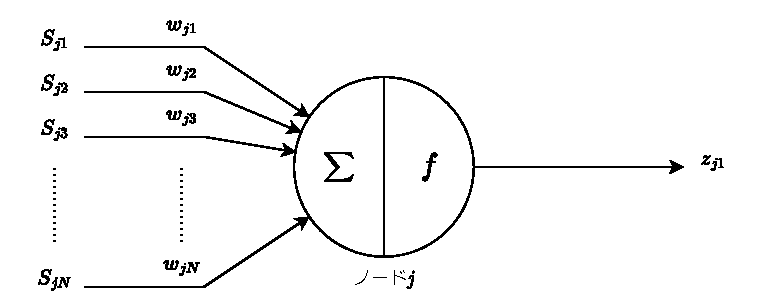
\includegraphics[scale=0.8]{img/expnode.pdf}
        \caption{シナプスとノードの関係}
    \end{center}
\end{figure}

ここでは,ノード $ j $ への $ N $ 個の入力 $ S_{1j}, S_{2j}, S_{3j}, ..., S_{Nj} $ に対して各々の重み $ w_{j1}, w_{j2}, w_{j3}, ..., w_{jN} $ となっている.この素子は入力とバイアス $ b_{j} $ を足した値 $ U_{j} $ を活性化関数 $ f_{j} $ の入力とし,活性化関数の出力をノードの出力 $ z_{j} $ とする.

\begin{equation}
    U_{j} = \sum_{i=1}^N S_{ji}w_{ji} + b_{j}
\end{equation}

\begin{equation}
    z_{j} = f_{j}(U_{j})
\end{equation}

このノードを組み合わせ,図2のような階層型ニューラルネットワークを考える.

\begin{figure}[h]
    \begin{center}
        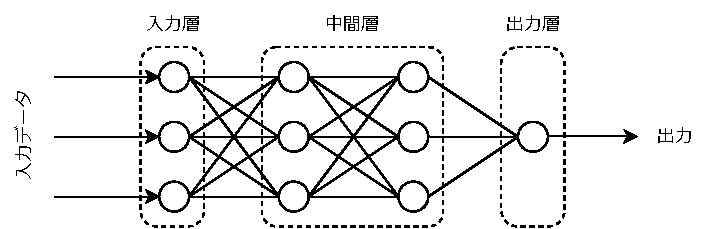
\includegraphics[scale=0.8]{img/forwardprop.pdf}
        \caption{階層型ニューラルネットワーク}
    \end{center}
\end{figure}

階層型ニューラルネットワークは,入力層,中間層,出力層からなり,まずタスクを解くための判断材料となる入力データが入力層のノードに入力される.中間層の入力はひとつ前の層の出力からなり,出力層の結果がネットワークの解答になる.

\clearpage
\subsection{活性化関数}
活性化関数は,与えられた入力をどのように活性化するかの動作を変更するものである.線形分離によって解くことができない問題に対しては,この活性化は非線形変換である必要がある\cite{活性化関数}.具体的には実数空間 $ V, W $ において  $ V $ から $ W $ への写像 $ f $ が以下の性質を満たさない変換である必要がある.ただし $ x, y \in V, c \in \mathbb{R} $ とする.

\begin{enumerate}
    \item 加法性: $ f(x + y) = f(x) + f(y) $ 
    \item 斉一次性: $ f(cx) = cf(x) $
\end{enumerate}

複数のノードの出力の合計をあるひとつノードとみなすことは線形変換に過ぎず,線形変換の繰り返しはその結果もまた線形性が保たれ,活性化関数を持たないネットワークは隠れ層を持つ場合と持たない場合で表現できる幅は変わらない.複数のニューロンからの入力の合計を活性化関数を通すことはネットワークがより多くの情報を表現できることを意味する.
代表的な活性化関数 $ f $ は次のようなものがある.

\begin{enumerate}
    \item ReLU関数
    \begin{equation}
        f(x) = 
        \begin{cases}
        x & (x > 0)\\
        0 & (x \leq 0)
        \end{cases}
    \end{equation}

    \item tanh関数
    \begin{equation}
        f(x) = \frac{e^{x} - e^{-x}}{e^{x} + e^{-x}}
    \end{equation}
\end{enumerate}

今回の実験では,これら2種類を含む10種類の活性化関数を用いる.